\chapter{Developer Documentation}

In this chapter I will explain what was my plan going into the development of my thesis, how I handled problems during development, and I will finally show the test conducted to compare the libraries.

\section{Development plan}

For my planing I choose to do my project using the \CC\ programming language. To visualize the data I choose to use \ac{SDL2} with \ac{ImGui} and OpenGL and obviously for \ac{GPGPU} libraries CUDA and OpenCL. The main plan was to implement the two edge detection algorithms. I could have choose to do only the algorithm implementation without a user interface but I decided against it. The reason simply being that goal of the thesis is to show the difference of \ac{GPGPU} libraries speed and be a helpful tool for people to test them out themselves. Thus the plan for the Gui was to have two programs one for synthetic testing environment pure library speed. The result from those test are for pictures that only contain two colors and have simple lines and curves on them. This proves a good way of testing for accuracy and speed but in a real world scenario a real picture could have very different results. Thus the other program's goal is to test real pictures. This program cannot test accuracy and it's main function is to test the speed of the algorithm on a real picture and show the results.


\subsection{Architecture and Classes}

The plan for the architecture was a simple Model View but its hard to differentiate what's part of a Model and View since there's no library elements or event management system in \CC\ and the aforementioned libraries. The plan was to write an abstraction layer over \ac{SDL2} to use as the base for displaying the \ac{ImGui} and the pictures. Obviously this contains some logic but these logic are mainly related to displaying the images and the Gui.

I will only describe the plans for the picture detector and will only go into the details of the synthetic tester when the plans differed because the basic structure of the two program is the same.

I will only explain the part of the plan for the View which is relevant to the thesis. I use my own \ac{SDL2}-OpenGl pipeline abstraction that is very generalised and could be changed to any library for example Qt to show images and the Gui. I choose to use my own abstraction because I wanted a light weight program and didn't want to depend on a huge library. 

\begin{figure}[H]
\centering
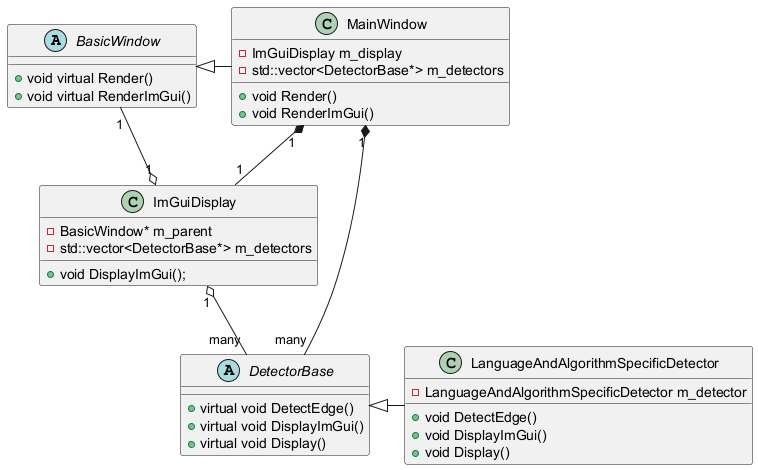
\includegraphics[width=0.8\linewidth]{view}
\caption{Class diagram of view plan}
\label{fig:class_view_plan}
\end{figure}

As I demonstrate in \autoref{fig:class_view_plan} the plan was that I have a basic abstract window class named \textit{BasicWindow} in my own pipeline abstraction and implement a main window from that. Because of the complexity of the ImGui display I choose to use a class to abstract out the common elements. Lastly the detectors themselves are implementing a base class so I can store them in the main window but still have different implementation for all the algorithms in all the languages. This means that I would have 6 of these classes because of this as I will show later in \autoref{chap:Imp_Arc} this changed while developing and I will explain the reason for it in that subsection. As I have stated above there was no plan for the synthetic tester to have different class structure so the only difference is how the ImGui looks.

As for the models architecturally I use the two libraries that I'm testing to implement the algorithms on the \ac{GPU} and I used no external libraries to implement the algorithm on the \ac{CPU}

\begin{figure}[H]
\centering
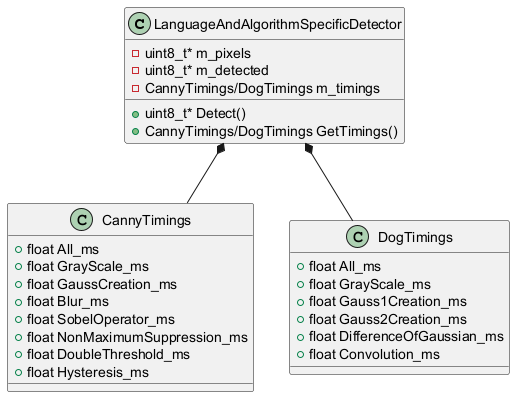
\includegraphics[width=0.8\linewidth]{model}
\caption{Class diagram of model plan}
\label{fig:class_model_plan}
\end{figure}

For the plan of the class structure because on CUDA I need separate functions, and for OpenCl I need separate kernel files, I thought that I cannot abstract out any common element except for the struct for the timings, I choose to just create separate classes for them. As shown on the Class diagram in \autoref{fig:class_model_plan} but as with the View as I started implementing it this planed changed slightly and I will discuss this latter at \autoref{chap:Imp_Arc}.

\subsection{Algorithms}
\label{chap:algo}

So far I only talked about my plans for the view and class structure but by an early stage I know which edge detection algorithms I want to implement and as I have already talked about in \autoref{chap:intro} they are: \ac{Canny} and \ac{DoG}. In this subsection I will demonstrate my plan for the algorithms.

\subsubsection{Canny edge detection}

According to the original article\cite{canny:paper} the \ac{Canny} algorithm has 4 steps

\begin{enumerate}[nolistsep]
\item Filter out any noise. The Gaussian filter is used for this purpose.
\item Find the intensity gradients of the image. For this purpose I use the Sobel filter.
\item Non-maximum suppression is applied. This removes pixels that are not considered to be part of an edge.
\item Hysteresis with double thresh holding. I choose to do this in two steps.
\end{enumerate}

The original article\cite{canny:paper} is very detailed but it's a hard read thus I used other sources\cite{canny:imp}\cite{canny:imp2} to understand the concept better and formulate the algorithms.

Firstly before I can do anything I have to grey scale the image. This is a very simple algorithm as shown in algorithm \ref{alg:grey} I just take the RGB pixel values and multiply them by 0.2999, 0.587, 0.114 accordingly,

\begin{algorithm}[H]
\caption{Grey scaling algorithm}
\label{alg:grey}
\begin{algorithmic}
\State \textbf{Data:} $I$ the RGB pixels of the image
\State \textbf{Result:} $I2$ the grey scaled value of the pixels
\For{$r \; g \; b$ pixel values in $I$ image}
\State $p = 0.299 * r + 0.587 * g + 0.114 * b$
\State where $p$ is the pixel value cores ponding in $I2$
\EndFor
\end{algorithmic}
\end{algorithm}

Now I can focus on the edge detection algorithm properly first is the Gaussian blur. I could use other blurring methods but this is the simplest for our purpose and I can later reuse this in the \ac{DoG} algorithm.

\begin{algorithm}[H]
\caption{Gaussian blur}
\label{alg:gauss}
\begin{algorithmic}
\State \textbf{Data:} $I$ the grey pixels of the image, $G$ the values in the Gaussian kernel in a matrix, $k$ is the size of the kernel
\State \textbf{Result:} $I2$ the output value of the pixels
\For{$c,r$ where $c$ is the index for the column and $r$ is the index for the row of the pixel in $I$ image}
\State $s = 0$
\For{$i=-\frac{k-1}{2},\ldots,\frac{k-1}{2}$}
\For{$j=-\frac{k-1}{2},\ldots,\frac{k-1}{2}$}
\State $s = I[c + i ][r + j] * G[i][j] + s $
\EndFor
\EndFor
\State $I2[c][r] = s$
\EndFor
\end{algorithmic}
\end{algorithm}

In the next step I'm going to calculate the intensity gradient and the edge direction for the image. This step is where I will final get edge lines before this I was only doing preliminary work. The gradient will be our edges and I can calculate the edge directions too which I will use in the next step when I do the Non-maximum suppression to find a single edge line. I use the two directional Sobel filters which are:
\[
\begin{bmatrix}
-1 & 0 & +1 \\
-2 & 0 & +2 \\
-1 & 0 & +1 \\
\end{bmatrix} \qquad
\begin{bmatrix}
+1 & +2 & +1 \\
0 & 0 & 0 \\
-1 & -2 & -1 \\
\end{bmatrix}
\]

\begin{algorithm}[H]
\caption{Intensity gradient}
\label{alg:sobel}
\begin{algorithmic}
\State \textbf{Data:} $I$ the pixels of the image
\State \textbf{Result:} $I2$ the intensity gradient value of the pixels, $I3$ is the edge direction of the pixels
\For{$c,r$ where $c$ is the index for the column and $r$ is the index for the row of the pixel in $I$ image}
\State $SX = \{-1, 0, +1, -2, 0, +2, -1, 0, +1\}$
\State $SY = \{+1, +2, +1, 0, 0, 0, -1, -2, -1\}$
\State $sx = 0$
\State $sy = 0$
\For{$i=-1,\ldots, 1$}
\For{$j=-1,\ldots, 1$}
\State $sx = I[c + i ][r + j] * SX[i][j] + sx $
\State $sy = I[c + i ][r + j] * SY[i][j] + sy $
\EndFor
\EndFor
\State $I2[c][r] = \sqrt{sx^2+sy^2}$
\State $t = \frac{\text{atan2}(sx,sy) * 180}{\pi} $
\If{$t < 180$}
\State $t = t + 180$
\EndIf
\State $I3[c][r] = t$
\EndFor
\end{algorithmic}
\end{algorithm}
\clearpage

Next comes the non maximum suppression in this step I will filter out the gradient so that only continuous edges remain for this purpose I will use the edge direction's I got from the previous step.

\begin{algorithm}[H]
\caption{Non-Maximum suppression}
\label{alg:max}
\begin{algorithmic}
\State \textbf{Data:} $I$ the intensity gradient of the image $I2$ the edge direction of the pixels 
\State \textbf{Result:} $I3$ the pixels of the image that only contain continuous edges
\For{$c,r$ where $c$ is the index for the column and $r$ is the index for the row of the pixel in $I$ image}
\State $q,r = 2000$
\If{$0 \leq I2[c][r] < 22.5$ or $157 \leq I2[c][r] \leq 180$}
\State $q = I[c][r + 1]$
\State $r = I[c][r - 1]$
\ElsIf{$22.5 \leq I2[c][r] < 67.5$}
\State $q = I[c + 1][r - 1]$
\State $r = I[c - 1][r + 1]$
\ElsIf{$67.5 \leq I2[c][r] < 112.5$}
\State $q = I[c + 1][r]$
\State $r = I[c - 1][r]$
\ElsIf{$112.5 \leq I2[c][r] < 157.5$}
\State $q = I[c - 1][r - 1]$
\State $r = I[c + 1][r + 1]$
\EndIf
\If{$I[c][r] \geq q$ and $I[c][r] \geq r$}
\State $I3[c][r] = I[c][r]$
\Else
\State $I3[c][r] = 0$
\EndIf
\EndFor
\end{algorithmic}
\end{algorithm}

The next step I choose to do separately into two separate because of the nature of the  algorithms but in reality they are just one the hysteresis. In the first step the double thresh holding where I categorize the edges into two groups weak edges and strong edges. Based on this then I take all the weak pixels and transform them into strong pixels only in the case when the week pixel have atleast one strong pixel sounding it.

\begin{algorithm}[H]
\caption{Double threshold}
\label{alg:thresh}
\begin{algorithmic}
\State \textbf{Data:} $I$ the pixels of the image, $l$ the low threshold, $h$ the high threshold
\State \textbf{Result:} $I2$ the week and strong pixels of the image
\For{$c,r$ where $c$ is the index for the column and $r$ is the index for the row of the pixel in $I$ image}
\If{$I[c][r] \geq h$}
\State $I2[c][r] = 255$
\ElsIf{$h > I[c][r] \geq l$}
\State $I2[c][r] = 125$
\Else
\State $I2[c][r] = 0$
\EndIf
\EndFor
\end{algorithmic}
\end{algorithm}

\begin{algorithm}[H]
\caption{Hysteresis}
\label{alg:hys}
\begin{algorithmic}
\State \textbf{Data:} $I$ the pixels of the image
\State \textbf{Result:} $I2$ the final image
\For{$c,r$ where $c$ is the index for the column and $r$ is the index for the row of the pixel where $I[c][r] = 125$}
\For{$i=-1,\ldots, 1$}
\For{$j=-1,\ldots, 1$}
\State $s =$ false
\If{$I[c + i][r + j] = 255 $}
\State $s$ = true
\EndIf
\EndFor
\EndFor
\If{$s =$ true}
\State $I[c][r] = 255$
\Else
\State $I[c][r] = 0$
\EndIf
\EndFor
\end{algorithmic}
\end{algorithm}

After I'm done with the Hysteresis I'm done with the algorithm and got my final picture.

\subsubsection{Difference of Gaussians}

This algorithm is much simpler then the previous while the \ac{Canny} have a lot of steps to get a fine tuned image it requires a per image fine tuning to get the best results. In comparison to that the \ac{DoG} algorithm requires much less fine toning but its less accurate too.

I basically already wrote the algorithm previously. First I use algorithm \ref{alg:grey} to gray scale the image. Than I only need algorithm \ref{alg:gauss} to use this. The only difference is that instead of supplying the algorithm a normal Gaussian kernel I first take the difference of two Gaussian kernels and I supply that kernel to the function. The resulting image will contain the edge lines of our image.

\section{Implementation}

\subsection{Architecture and Classes}
\label{chap:Imp_Arc}



\section{Testing}
\label{chap:dev_testing}

My plans for the testing is simple. Since both programs is designed in a way to compare the algorithms and libraries I will just use them to test the code. Since the visualization is very rudimentary and the code for it is is even simpler there's no need for it to be tested. There's only one vector of failure is that if someone deletes one of the pre defined pictures, OpenCl kernels or OpenGl shaders. These are assumed to exists at all time since the programs cannot function without it.

\subsection{Real picture tester}

First I will show results about the real picture tester since it is more focused on the visual aspects and not hard data like the synthetic tester. My plans for testing this is to compare bot \ac{DoG} and \ac{Canny} algorithms in all three implementations based on how they look and what we can see as differences and how much time it takes them. As I have mentioned in \autoref{chap:real_pic_tester} I only used pre defined pictures the sizes and names of the pictures are shown below in \autoref{tab:pictures}. I will only show timings if they are relevant but how picture and settings size effect timing will be discussed in \autoref{chap:test_synt_test}.

\begin{table}[H]
\centering
\begin{tabular}{| c | c | c |}
\hline
Name & Width & Height \\
\hline \hline	
gem & 2560 & 1440 \\
\hline
house & 1600 & 1200 \\
\hline
monkey & 7680 & 4320 \\
\hline
lines & 100 & 100 \\
\hline
\end{tabular}
\caption{Pictures used and their sizes}
\label{tab:pictures}
\end{table}

\begin{figure}[H]
\centering
\begin{minipage}[t]{.49\textwidth}
\centering
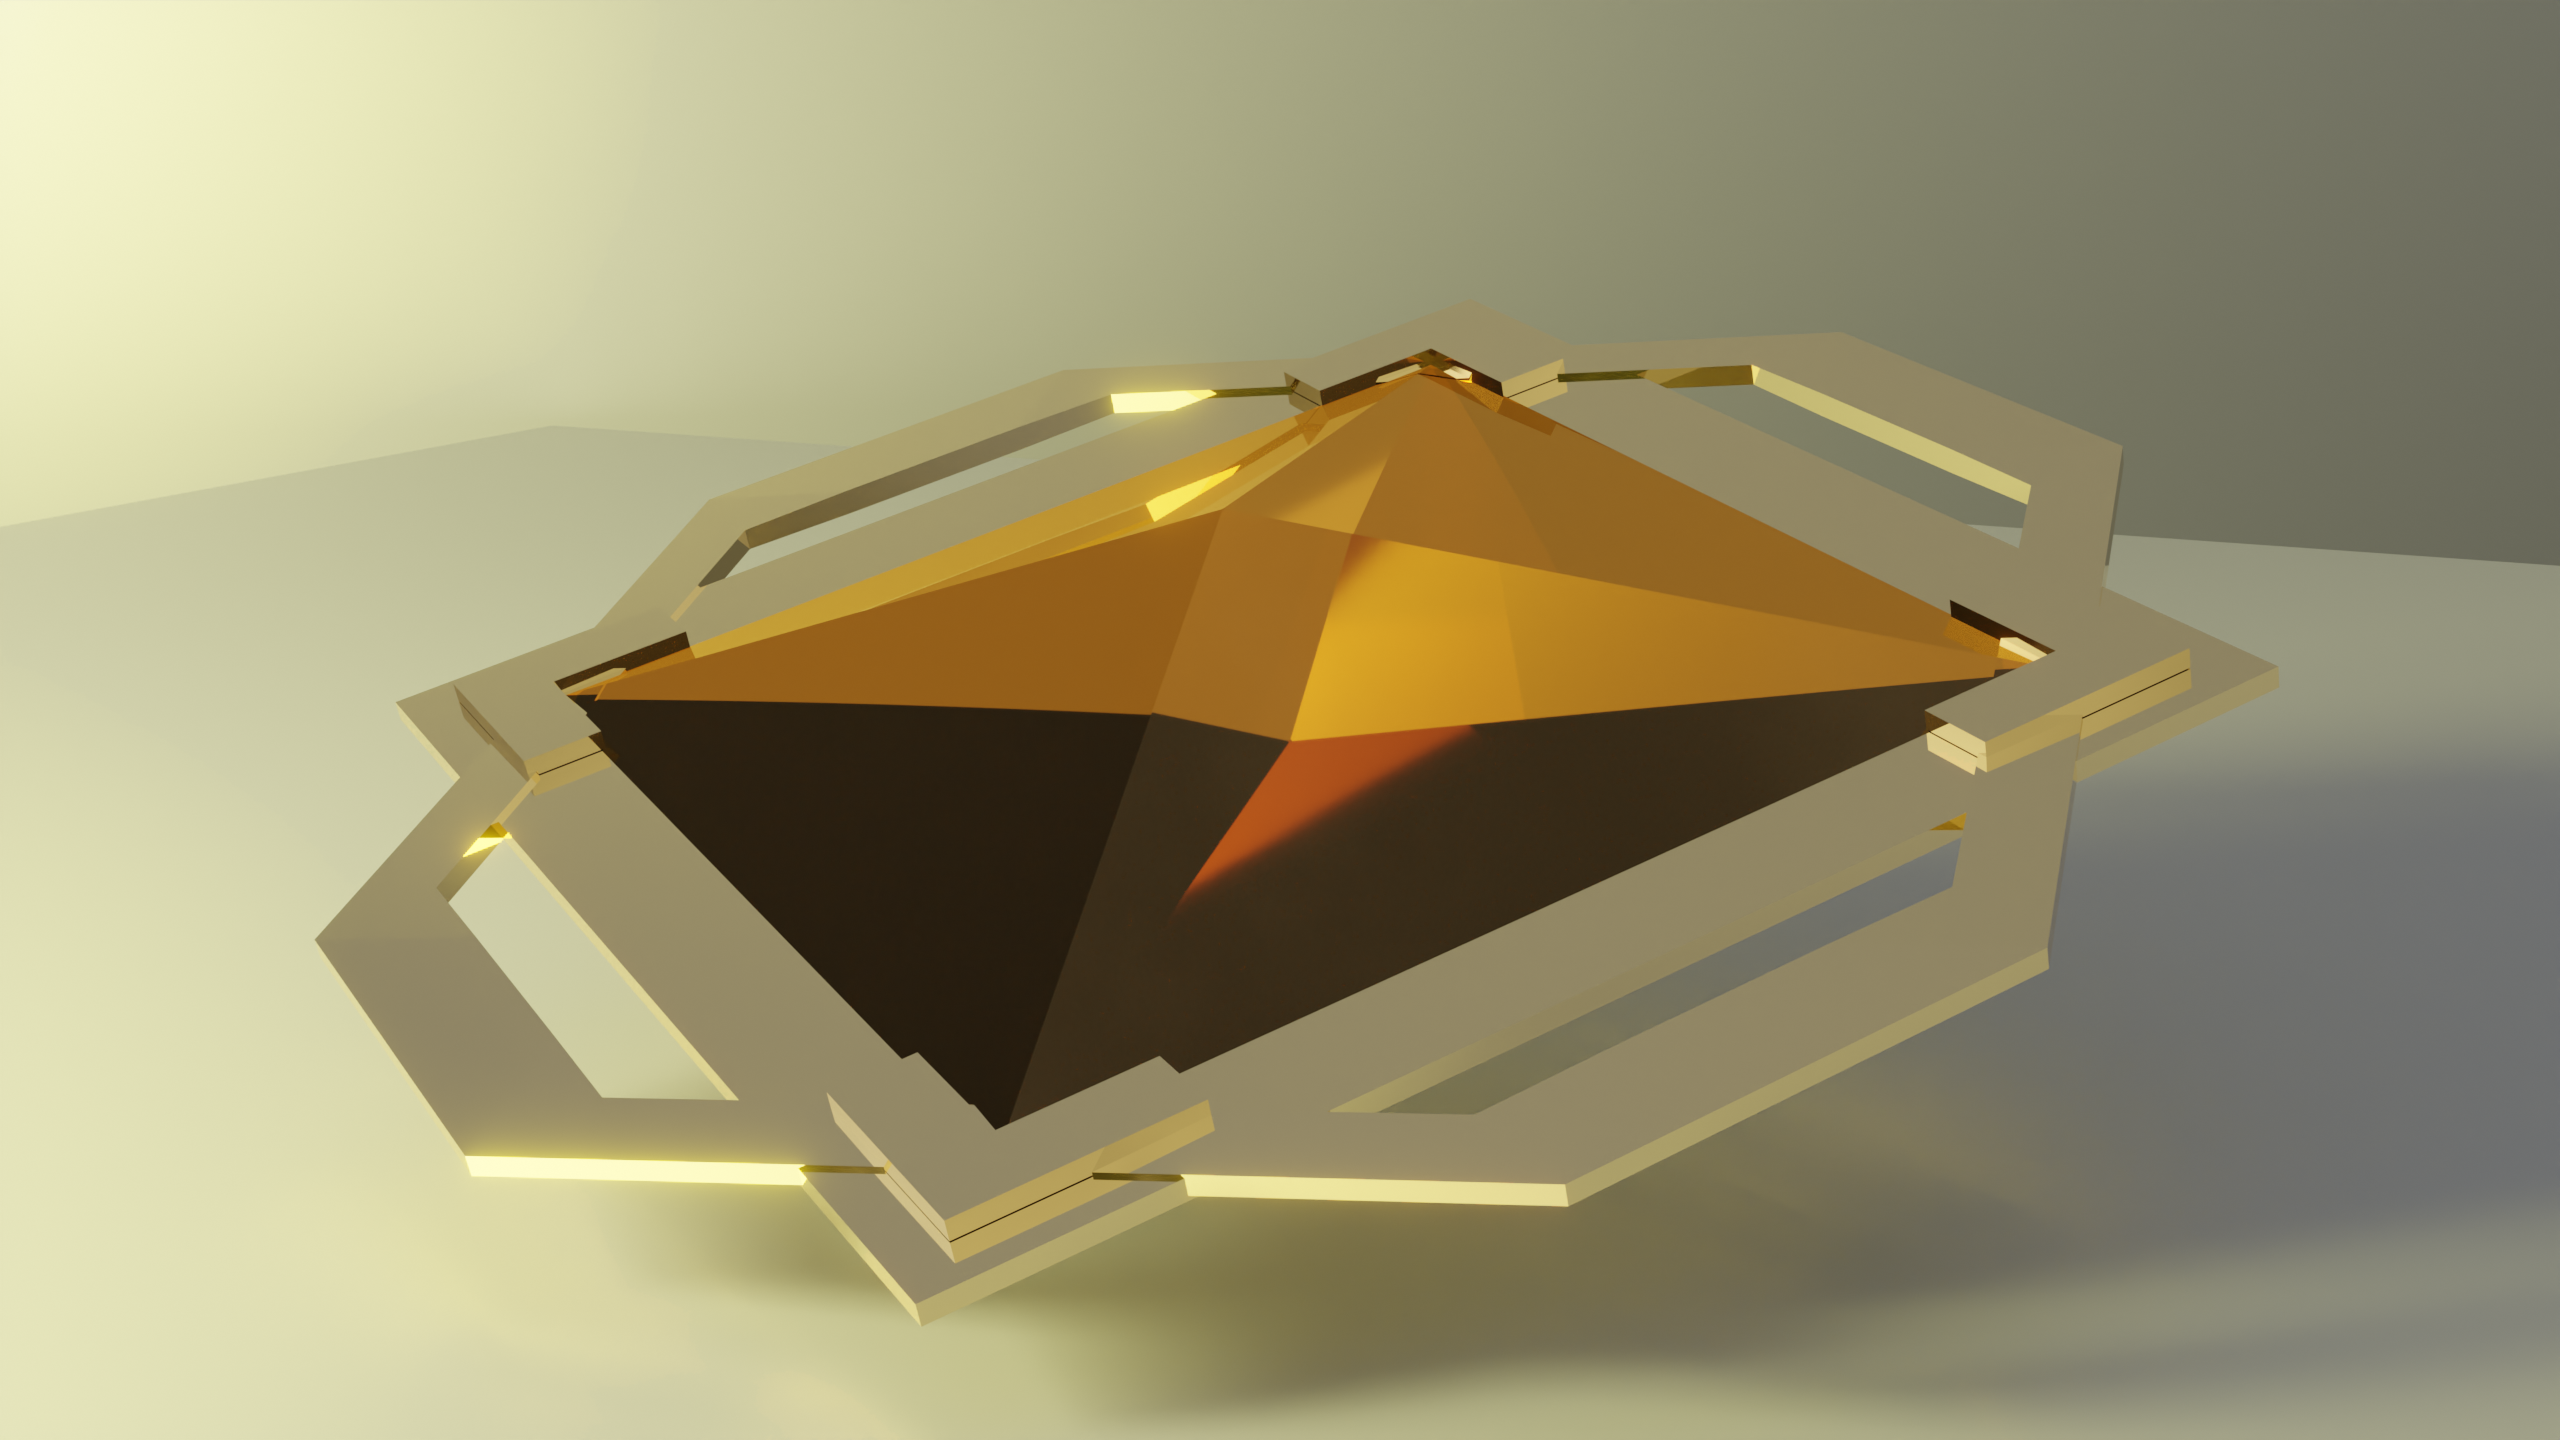
\includegraphics[width=\linewidth]{gem}
\addtocounter{figure}{-1}
\captionsetup{labelformat=empty}
\caption{gem}
\end{minipage}
\begin{minipage}[t]{.49\textwidth}
\centering
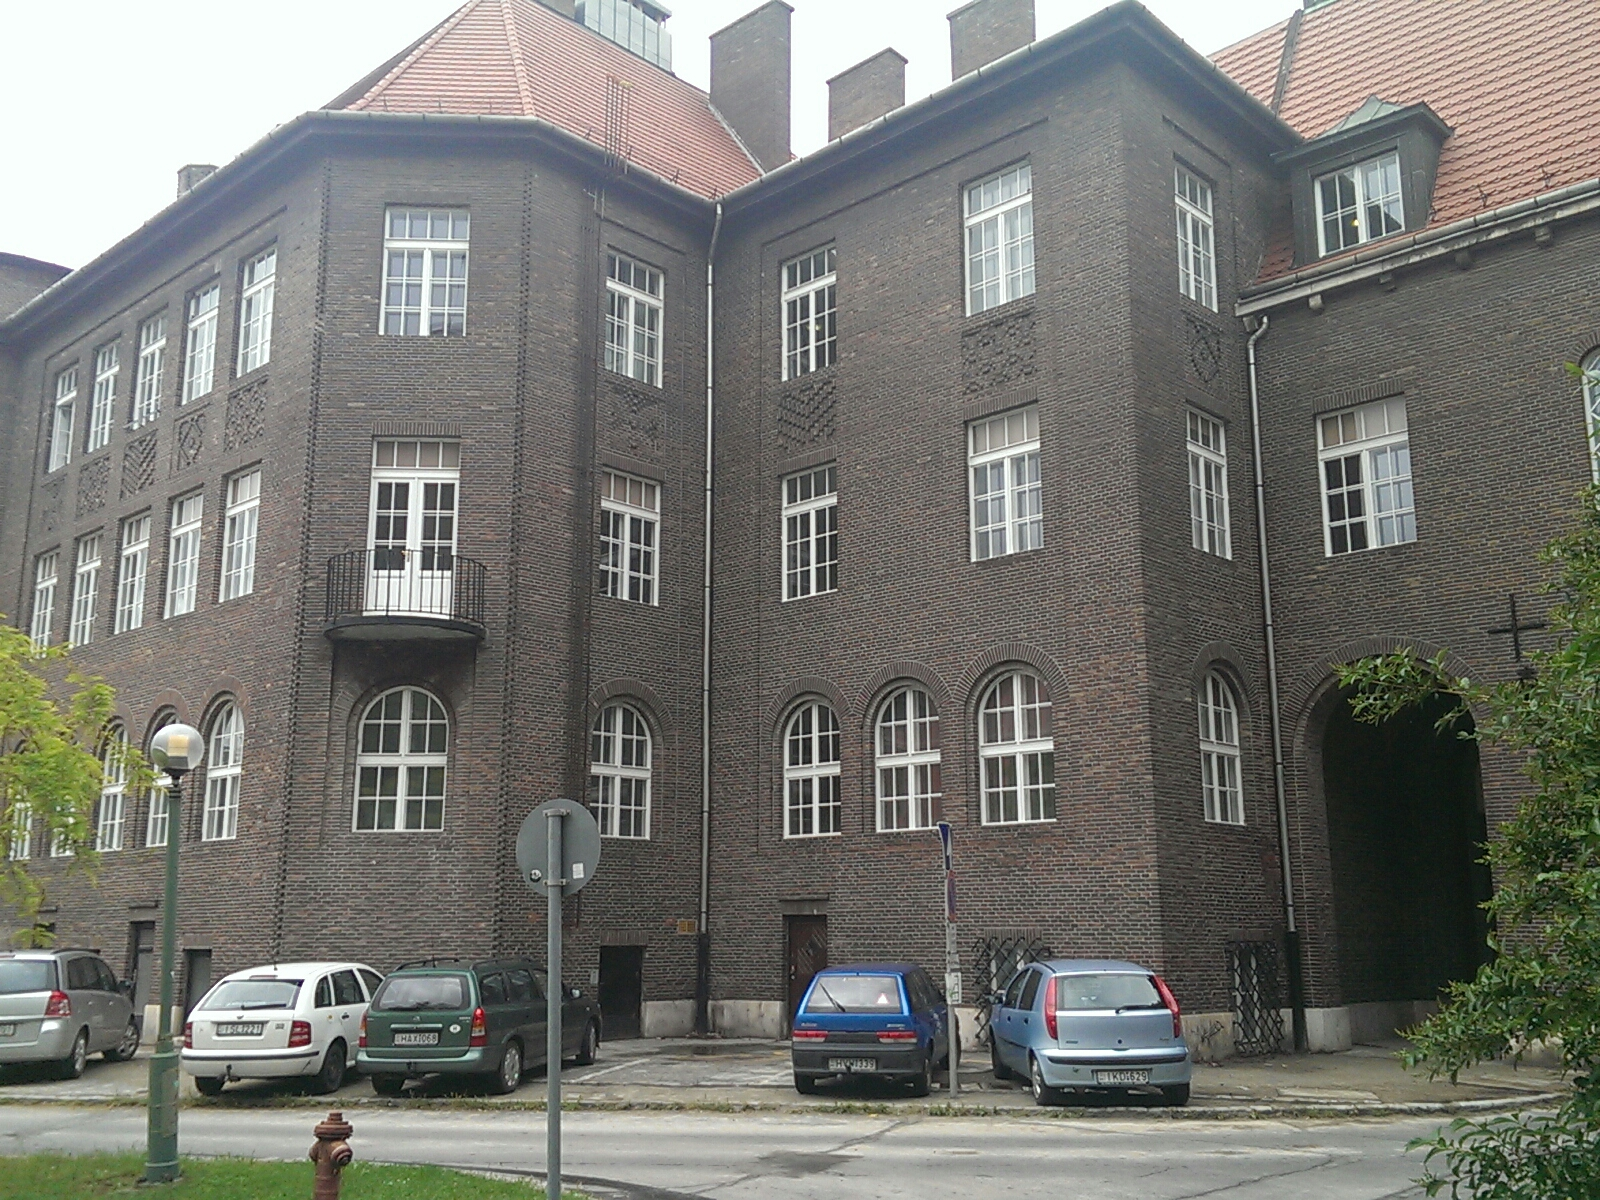
\includegraphics[width=\linewidth]{house}
\addtocounter{figure}{-1}
\captionsetup{labelformat=empty}
\caption{house}
\end{minipage}
\begin{minipage}[t]{.49\textwidth}
\centering
\includegraphics[width=\linewidth]{monkey}
\addtocounter{figure}{-1}
\captionsetup{labelformat=empty}
\caption{monkey}
\end{minipage}
\begin{minipage}[t]{.49\textwidth}
\centering
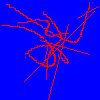
\includegraphics[width=\linewidth, height=.85\linewidth]{lines}
\addtocounter{figure}{-1}
\captionsetup{labelformat=empty}
\caption{lines}
\end{minipage}
\caption{The pictures base}
\label{fig:pictures}
\end{figure}

 For this reason I have done quiet a numerous test show in \autoref{tab:real_pic_canny} and \autoref{tab:real_pic_dog}. In the tables I show which picture I used and what settings I set for all three implementations.

\begin{table}[H]
\centering
\resizebox{\textwidth}{!}{\begin{tabular}{| c | c | c | c | c | c |}
\hline
&Name & Gauss kernel size & Standard deviation & High Threshold & Low Threshold\\
\hline\hline
1 & lines & $3$ & $1.0$ & $20.0$ & $10.0$ \\ 
\hline
\end{tabular}}
\caption{Test plans for the Real picture tester for \ac{Canny} algorithm}
\label{tab:real_pic_canny}
\end{table}

\begin{table}[H]
\centering
\resizebox{\textwidth}{!}{\begin{tabular}{| c | c | c | c | c |}
\hline
& Name & Gauss kernel size & Standard deviation one & Standard deviation two \\
\hline \hline
1 & lines & $7$ & $0.1$ & $10.0$ \\
\hline
\end{tabular}}
\caption{Test plans for the Real picture tester for \ac{DoG} algorithm}
\label{tab:real_pic_dog}
\end{table}

The tests in both algorithms case serve to show the same difference so I will explain both of them tougher. The first test is to show what the algorithm looks like exactly this is show in \autoref{fig:test1}. The slight color difference we can detect in the \ac{DoG} algorithm is because of floating point precisions.


\begin{figure}[H]
\centering
\begin{minipage}[t]{.325\textwidth}
\centering
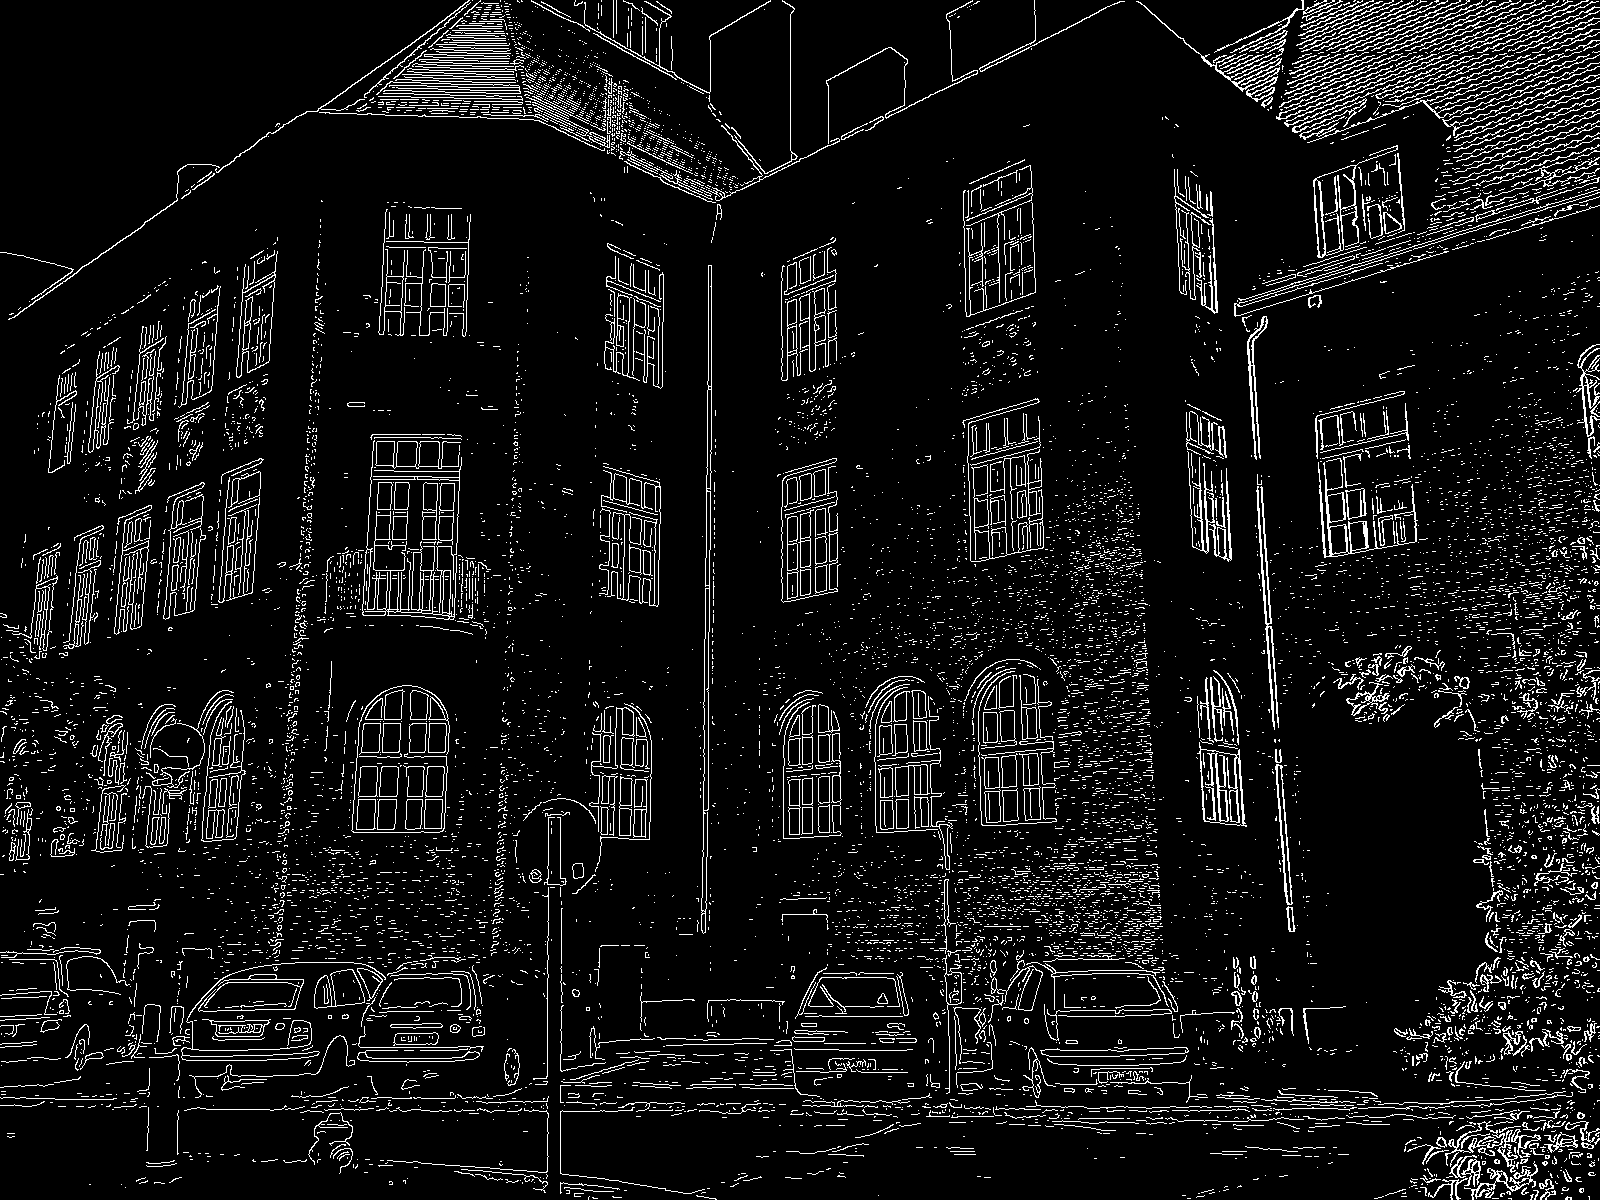
\includegraphics[width=\linewidth]{test1/canny_cpu}
\addtocounter{figure}{-1}
\captionsetup{labelformat=empty}
\caption{Cpu Canny}
\end{minipage}
\begin{minipage}[t]{.325\textwidth}
\centering
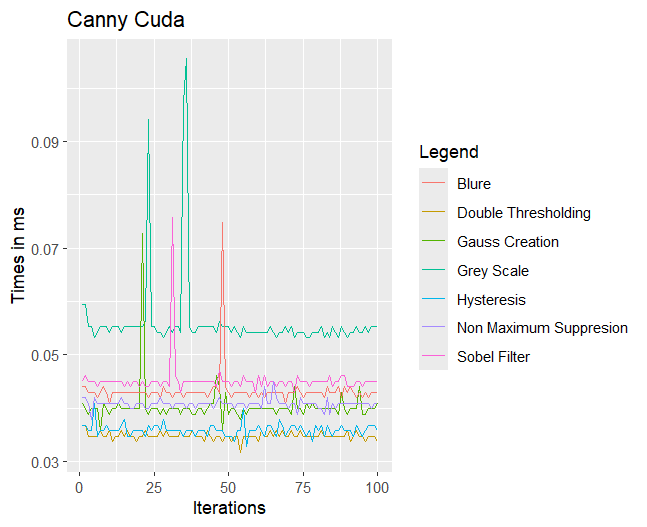
\includegraphics[width=\linewidth]{test1/canny_cuda}
\addtocounter{figure}{-1}
\captionsetup{labelformat=empty}
\caption{Cuda Canny}
\end{minipage}
\begin{minipage}[t]{.325\textwidth}
\centering
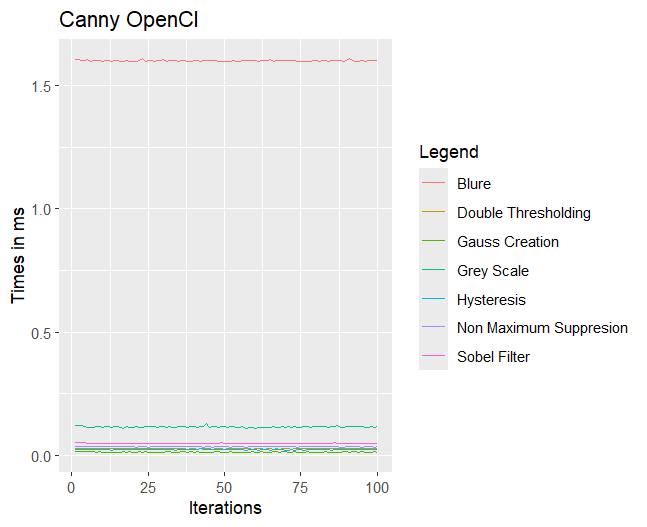
\includegraphics[width=\linewidth]{test1/canny_open_cl}
\addtocounter{figure}{-1}
\captionsetup{labelformat=empty}
\caption{OpenCl Canny}
\end{minipage}
\begin{minipage}[t]{.325\textwidth}
\centering
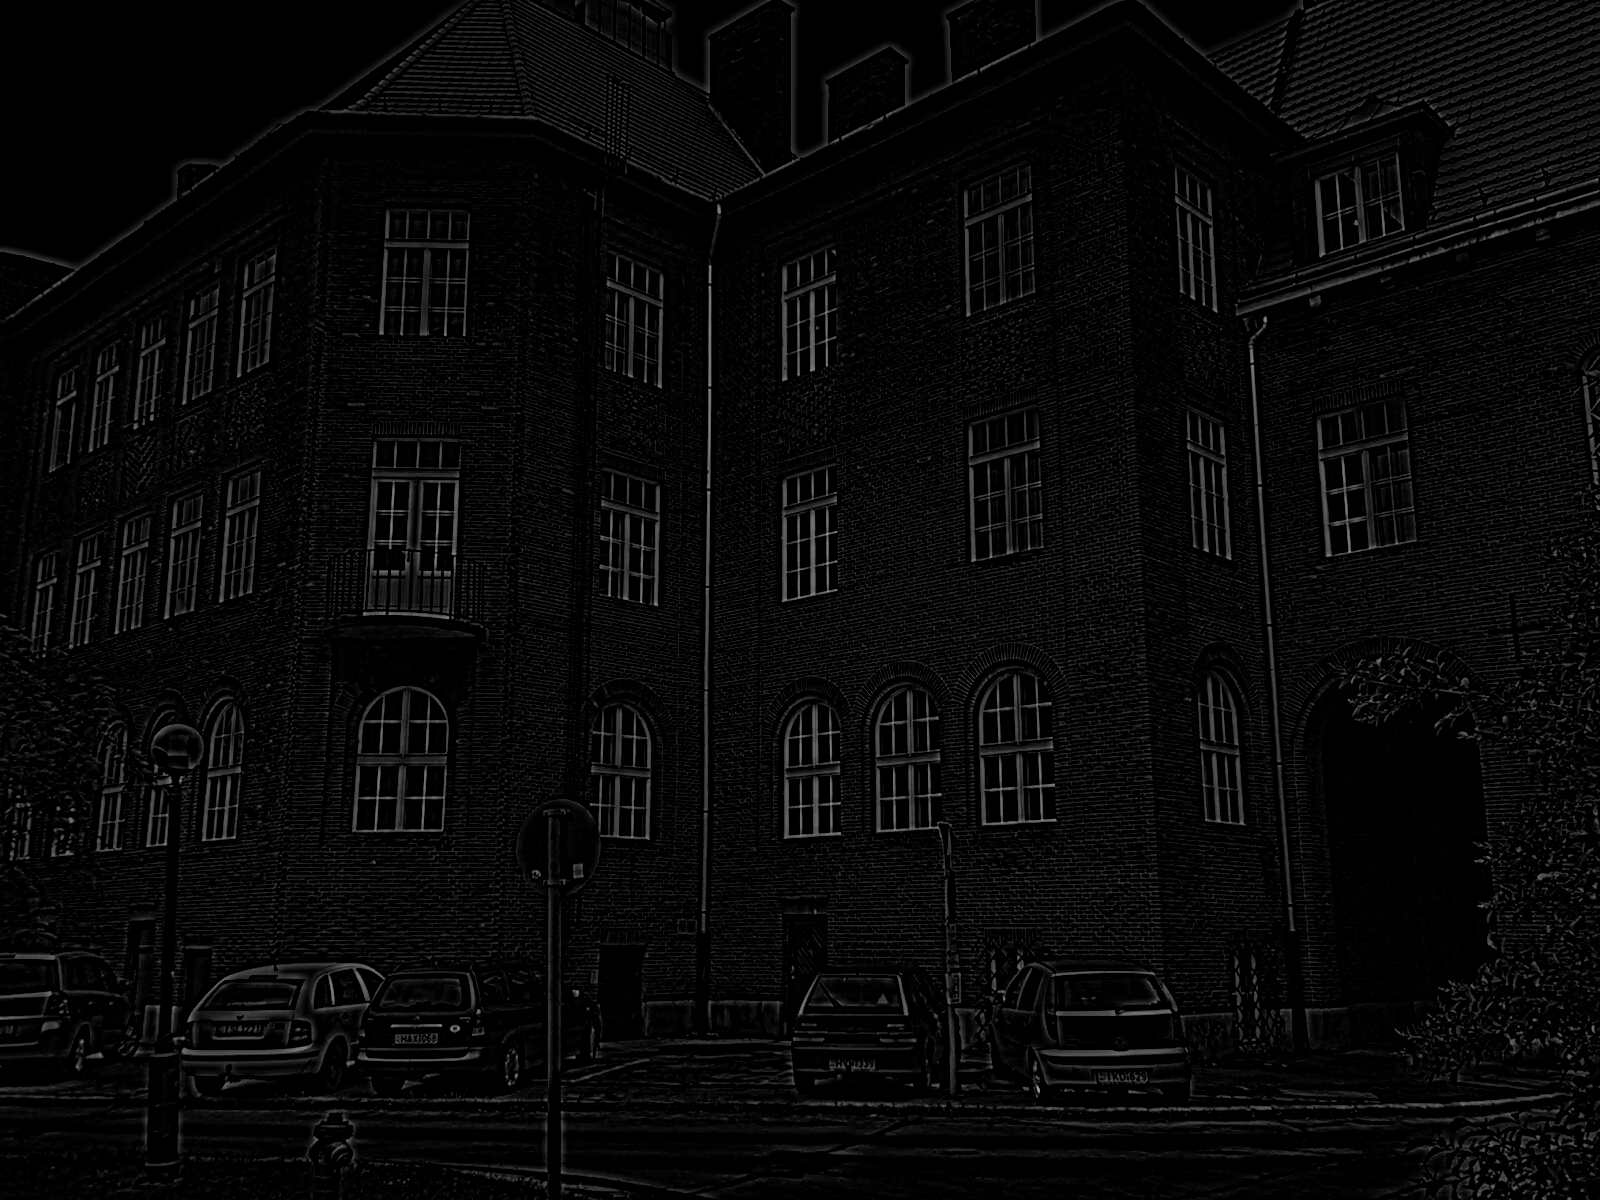
\includegraphics[width=\linewidth]{test1/dog_cpu}
\addtocounter{figure}{-1}
\captionsetup{labelformat=empty}
\caption{Cpu DoG}
\end{minipage}
\begin{minipage}[t]{.325\textwidth}
\centering
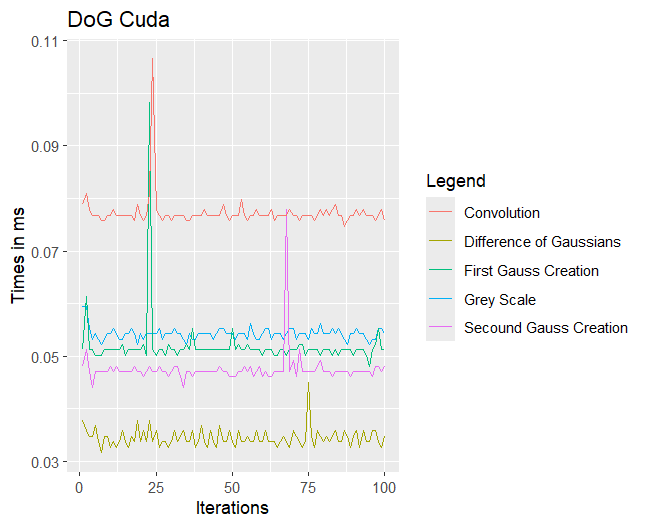
\includegraphics[width=\linewidth]{test1/dog_cuda}
\addtocounter{figure}{-1}
\captionsetup{labelformat=empty}
\caption{Cuda DoG}
\end{minipage}
\begin{minipage}[t]{.325\textwidth}
\centering
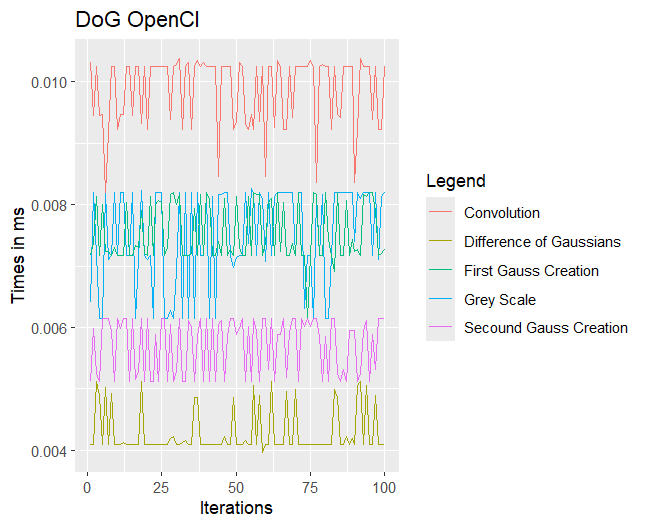
\includegraphics[width=\linewidth]{test1/dog_open_cl}
\addtocounter{figure}{-1}
\captionsetup{labelformat=empty}
\caption{OpenCl DoG}
\end{minipage}
\caption{Pictures of the first test for real pictures}
\label{fig:test1c}
\end{figure}


\begin{table}[H]
\centering
\resizebox{\textwidth}{!}{\begin{tabular}{| c | c | c | c | c | c | c | c | c |}
\hline
Name & Whole & Grey & Gauss & Blur & Sobel & Non Max & Threshold & Hysteresis \\
\hline \hline
Cpu Canny& $3.517$ & $0.0525$ & $0.0065$ & $1.1203$ & $1.9339$ & $0.1452$ & $0.0548$ & $0.038$ \\
\hline
Cuda Canny& $1.10387$ & $0.095232$ & $0.042784$ & $0.047104$ & $0.410624$ & $0.04288$ & $0.0408$ & $0.053248$ \\
\hline
OpenCl Canny& $9.7643$ & $0.00816$ & $0.006144$ & $0.005184$ & $0.006144$ & $0.006144$ & $0.006144$ & $0.00416$\\
\hline
\end{tabular}}
\resizebox{\textwidth}{!}{\begin{tabular}{| c | c | c | c | c | c | c |}
\hline
Name & Whole & Grey & Gauss creation 1 & Gauss creation 2 & DoG & Convolution \\
\hline \hline
Cpu DoG& $6.3464$ & $0.0478$ & $0.0056$ & $0.001$ & $0.0003$ & $6.0298$  
 \\
\hline
Cuda DoG& $0.83456$ & $0.16384$ & $0.044032$ & $0.014336$ & $0.25904$ & $0.062464$  
 \\
\hline
OpenCl DoG&$4.4794$ & $4.155$ & $0.0661$ & $0.0414$ & $0.0577$ & $0.0599$ 
\\
\hline
\end{tabular}}
\caption{Timings of the first test for real pictures}
\label{tab:test1c}
\end{table}

The first thing to note is that the OpenCl timings will look strange. That's because I used the platform specific timing functions in every case and while Cuda offers a timing method with events. OpenCl on the other hand only offers method to time the execution time of a kernel. This results in the unfortunate fact that the timing whole execution is impossible with platform specific method. For this reason I choose to time it with the chorons built in \CC\ library but this includes the time it took for the kernel to start and other synchronization and function call timing.


\subsection{Synthetic tester}
\label{chap:test_synt_test}

As for the synthetic tester I will now focus on what effects the size of the picture and the kernel size has on execution time. And I will show what effect does someone's machine has on the program. Lastly what we can say about the error rate of these algorithms and their accuracy. Just like previously all the tests are listed below in \autoref{tab:sync_pic_canny} and \autoref{tab:sync_pic_dog}.
\begin{table}[H]
\centering
\resizebox{\textwidth}{!}{\begin{tabular}{| c | c | c | c | c | c | c |}
\hline
&Iterations & Width $\times$ Height & Gauss kernel size & Standard deviation & High Threshold & Low Threshold\\
\hline\hline
1 & 100& $100\times 100$st & $3$ & $1.0$ & $20.0$ & $10.0$ \\ 
\hline
\end{tabular}}
\caption{Test plans for the  Synthetic tester for \ac{Canny} algorithm}
\label{tab:sync_pic_canny}
\end{table}

\begin{figure}[H]
\centering
\begin{minipage}[t]{.325\textwidth}
\centering
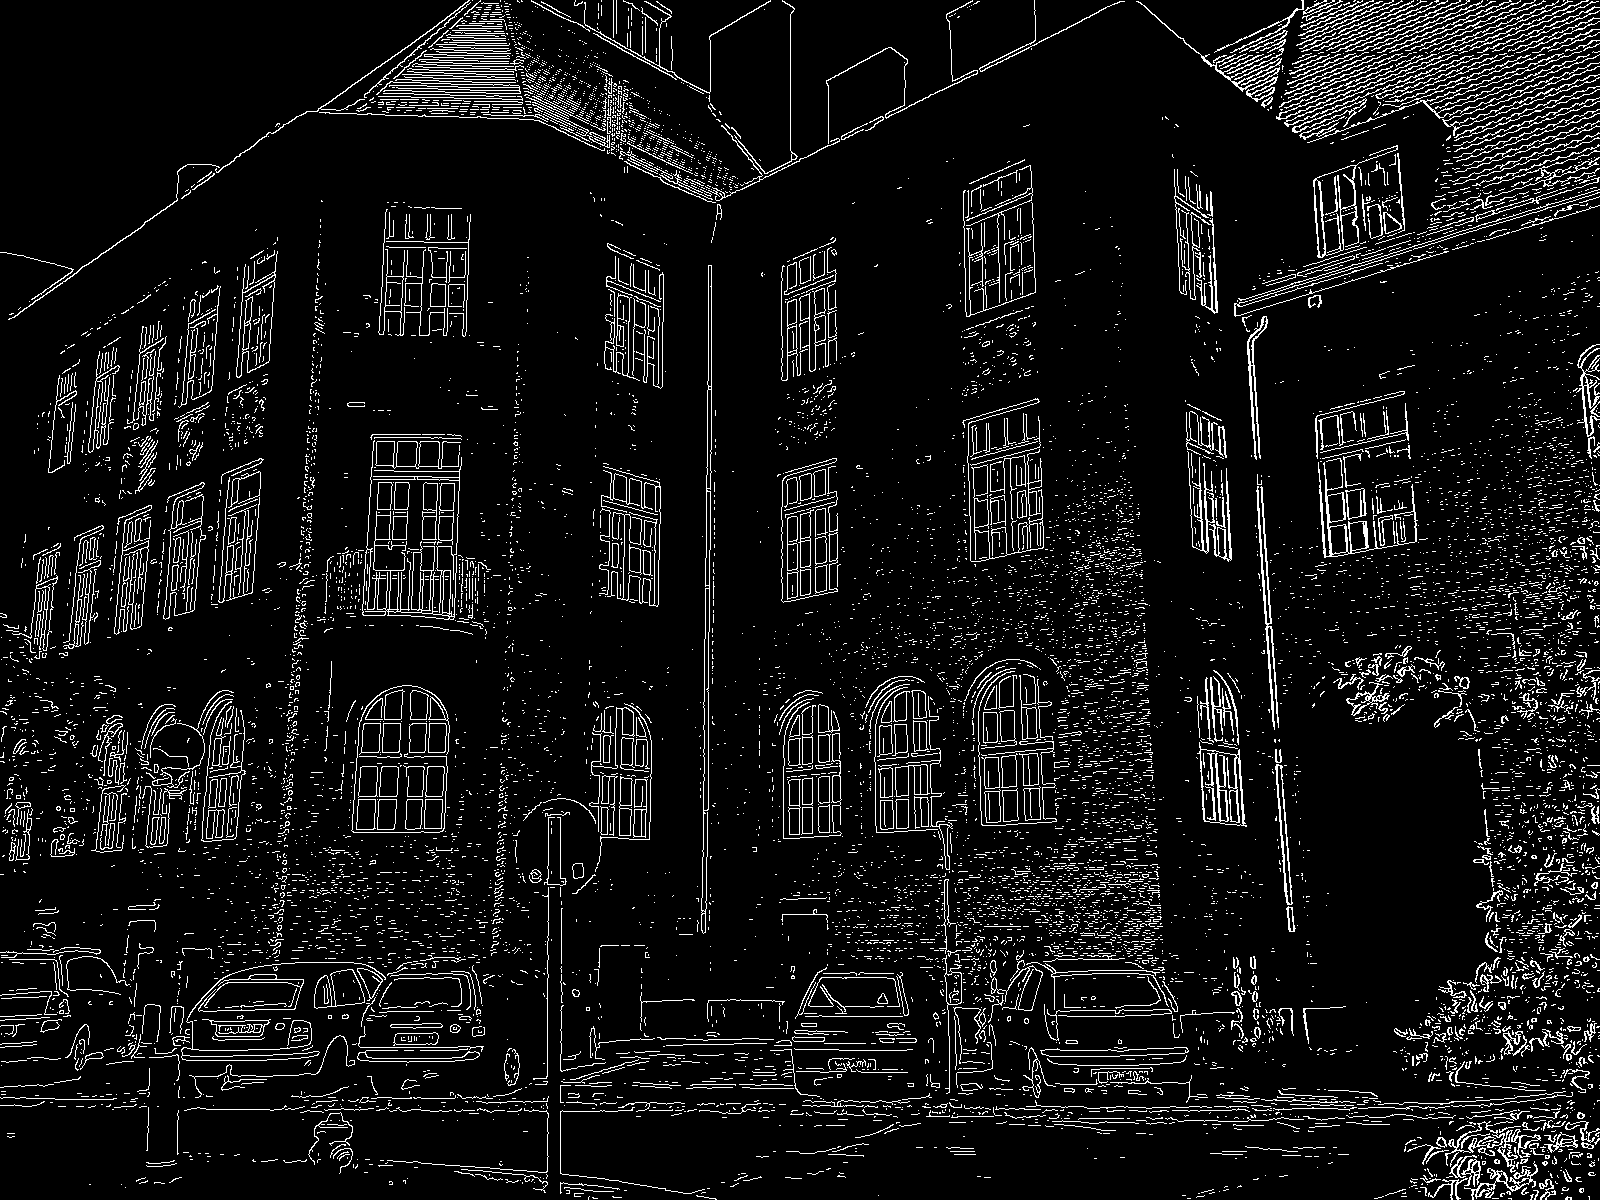
\includegraphics[width=\linewidth]{test1/canny_cpu}
\addtocounter{figure}{-1}
\captionsetup{labelformat=empty}
\caption{Cpu Canny}
\end{minipage}
\begin{minipage}[t]{.325\textwidth}
\centering
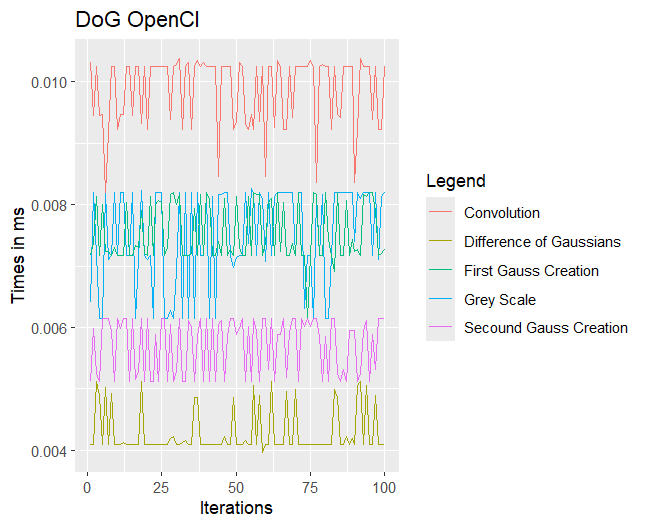
\includegraphics[width=\linewidth]{test1/dog_open_cl}
\addtocounter{figure}{-1}
\captionsetup{labelformat=empty}
\caption{Cuda Canny}
\end{minipage}
\begin{minipage}[t]{.325\textwidth}
\centering
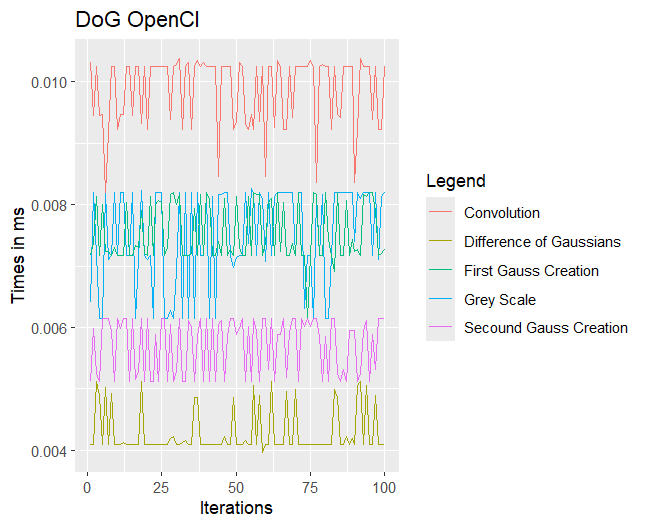
\includegraphics[width=\linewidth]{test1/dog_open_cl}
\addtocounter{figure}{-1}
\captionsetup{labelformat=empty}
\caption{OpenCl Canny}
\end{minipage}
\begin{minipage}[t]{.325\textwidth}
\centering
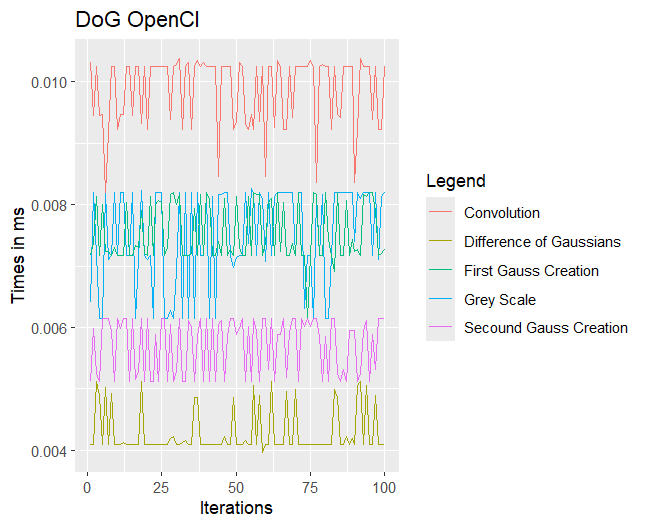
\includegraphics[width=\linewidth]{test1/dog_open_cl}
\addtocounter{figure}{-1}
\captionsetup{labelformat=empty}
\caption{Cpu DoG}
\end{minipage}
\begin{minipage}[t]{.325\textwidth}
\centering
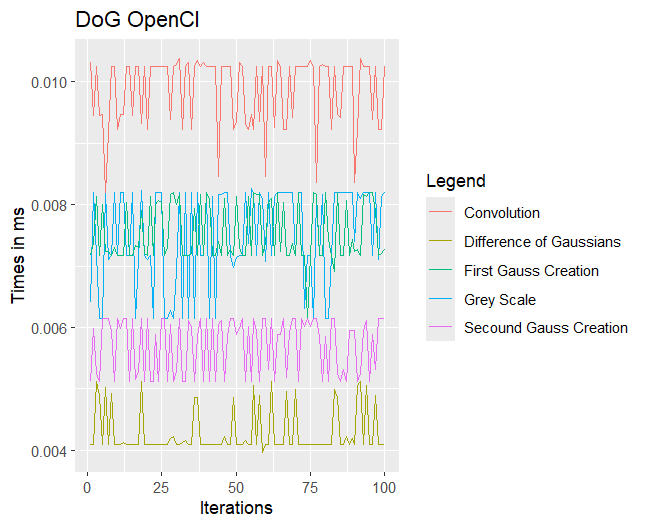
\includegraphics[width=\linewidth]{test1/dog_open_cl}
\addtocounter{figure}{-1}
\captionsetup{labelformat=empty}
\caption{Cuda DoG}
\end{minipage}
\begin{minipage}[t]{.325\textwidth}
\centering
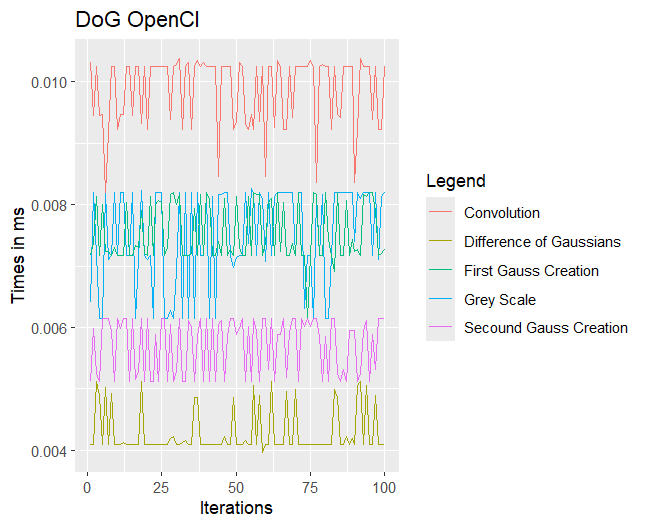
\includegraphics[width=\linewidth]{test1/dog_open_cl}
\addtocounter{figure}{-1}
\captionsetup{labelformat=empty}
\caption{OpenCl DoG}
\end{minipage}
\caption{Pictures of the first test for real pictures}
\label{fig:test1d}
\end{figure}
